\documentclass[crop,tikz]{standalone}

% Čech nerve is, up to homotopy, invariant to duplicating a point.

\begin{document}
	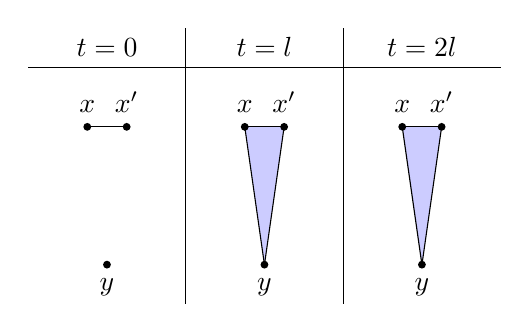
\begin{tikzpicture}
	\node[label=above:{$t=0$}] at (0.25, .4) {};
	\draw (0,-0.25) -- (0.5,-0.25);
	\node[circle,inner sep=1pt,fill=black,label=above:{$x$}] at (0,-0.25) {};
	\node[circle,inner sep=1pt,fill=black,label=above:{$x'$}] at (0.5,-0.25) {};
	\node[circle,inner sep=1pt,fill=black,label=below:{$y$}] at (0.25,-2) {};

	
	\draw (1.25,1) -- (1.25,-2.5);
	

	\node[label=above:{$t=l$}] at (2.25, .4) {};
	\fill[fill=blue!20] (2,-0.25) -- (2.5,-0.25) -- (2.25,-2);
	\draw (2,-0.25) -- (2.5,-0.25);
	\draw (2,-0.25) -- (2.25,-2);
	\draw (2.5,-0.25) -- (2.25,-2);
	\node[circle,inner sep=1pt,fill=black,label=above:{$x$}] at (2,-0.25) {};
	\node[circle,inner sep=1pt,fill=black,label=above:{$x'$}] at (2.5,-0.25) {};
	\node[circle,inner sep=1pt,fill=black,label=below:{$y$}] at (2.25,-2) {};

	
	\draw (3.25,1) -- (3.25,-2.5);
	
	
	\node[label=above:{$t=2l$}] at (4.25, .4) {};
	\fill[fill=blue!20] (4,-0.25) -- (4.5,-0.25) -- (4.25,-2);
	\draw (4,-0.25) -- (4.5,-0.25);
	\draw (4,-0.25) -- (4.25,-2);
	\draw (4.5,-0.25) -- (4.25,-2);
	\node[circle,inner sep=1pt,fill=black,label=above:{$x$}] at (4,-0.25) {};
	\node[circle,inner sep=1pt,fill=black,label=above:{$x'$}] at (4.5,-0.25) {};
	\node[circle,inner sep=1pt,fill=black,label=below:{$y$}] at (4.25,-2) {};
	
	
	\draw (-0.75,0.5) -- (5.25,0.5);
	\end{tikzpicture}
\end{document}